%%%%%%%%%%%%%%%%%%%%%%%%%%%%%%%%%%%%%%%%%%%%
%%% INSCRIPTION
%%%%%%%%%%%%%%%%%%%%%%%%%%%%%%%%%%%%%%%%%%%%



\mysection{Inscription}{research-inscription}

Inscription is the catch-all the written words, incantations, symbols, and engravings that allow Philosophers to capture and control Arcana.  Practicing Inscription requires the Settlement where you're taking the Vacation to have a Library (see the Core Rules). Inscription is divided into 3 groups:

\mybullet{
  \item \mylink{Transcription}{research-inscription-transcription}: Writing magical texts to Fetishes and Grimoires
  \item \mylink{Tattoo}{research-inscription-tattoo}: Branding and marking the flesh of living things with magical symbols
  \item \mylink{Sigils}{research-inscription-sigils}: Etching and scribing magical runes
}

  \begin{center}
  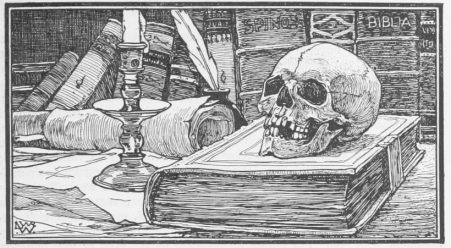
\includegraphics[scale=.5]{Inscription_1}
  \end{center}



\mysubsection{Transcription}{research-inscription-transcription}

Transcription is used to: 
\mybullet {
  \item prepare a new Grimoire so that it "belongs" to you; or
  \item defuse a Grimoire you've stolen from another wizard; or
  \item scribe a spell from a Fetish into a Grimoire; or
  \item scribe a spell from your Grimoire to a Fetish
}

\myhighlight{Preparing Grimoires}{inscription-preparing-grimoires}

By purchasing a blank Grimoire and placing one or more \mylink{Wizard Sigils}{research-sigil-wizard} on it, the Grimoire becomes yours and can now have spells written into it with Scribing (see below).  It is also trapped and needs to be defused in order to be read by another.   You can place as many Wizard Sigils on your Grimoire(s) as you can afford, making them harder to defuse. You can add additional Wizard Sigils at any time during a Vacation.

\myhighlight{Defusing Grimoires}{inscription-defusing-grimoires}

In order to read another sorcerer's Grimoire, you must defuse the traps inside.  You must spend a Research for every Wizard Sigil on the Grimoire.  You don't have to remove all the Sigils at once i.e. you can spread it out over multiple Vacations.  You can read a Grimoire even if it's trapped, but that sets the traps off (this removes the Sigil(s), however).  If you set the trap off, roll on \mylink{Grimoire Traps}{grimoire-traps} once for each Sigil.  Sigils can be removed through other means (like the Knave Virtue "Whispers of Sun Wukong", or by placing the sorcerer's finger on the Sigil and speaking its "true name").

Each Sigil removed is an Iron craft (1 Research; 100\FE).

\myhighlight{Scribing: Fetish to Grimoire}{inscription-scribing-fetish-to-grimoire}

You can write a spell from a Fetish (including a Philosopher's skull) to your Grimoire.  Doing so erases the spell from the Fetish or skull no matter how many \UD it had remaining.  Scribing a spell into your Grimoire is an Iron craft (1 Research; 100\FE)

\myhighlight{Scribing: Grimoire to Fetish}{inscription-scribing-grimoire-to-fetish}

You copy a spell you know (from a Grimoire, Fetish, or your head) to a Fetish.  The Fetish can be a papyrus, set of mouse skulls, handle of an axe, roll of snakeskin, etc. etc.  The item can't be living (that would be a Tattoo) but can be anything you desire.  A Fetish can only have a single spell on it.  All Fetishes have a \UD of d4 - when the \UD is exhausted, the magical words disappear from the Fetish.  You cast spells from the Fetish using your Blood \POOL, OR you may forgo the Blood die and roll a single d6 for the effect.  You still roll the \UD for the Fetish either way.

Creating a Fetish is an Iron craft (1 Research; 100\FE)


\mysubsection{Tattoo}{research-inscription-tattoo}

Tattoos can be inscribed on the body as specified below.  Creating a tattoo is a Silver craft (3 Research; 300\AG).  You can't move a tattoo from yourself to someone else - the tattoo stays with the person.  The tattoos below are the most common, but work out with the Arbiter if you want something more esoteric ...

\myhighlight{Dagger (Limb)}{sorcerer-tattoo-dagger}

Touching the dagger immediately brings it into your hand.  Place the dagger back on the limb returns it to being a tattoo.  The dagger is normal in all ways.

\myhighlight{Torch (Limb)}{sorcerer-tattoo-torch}

As dagger above.  The torch never goes out.

  \begin{center}
  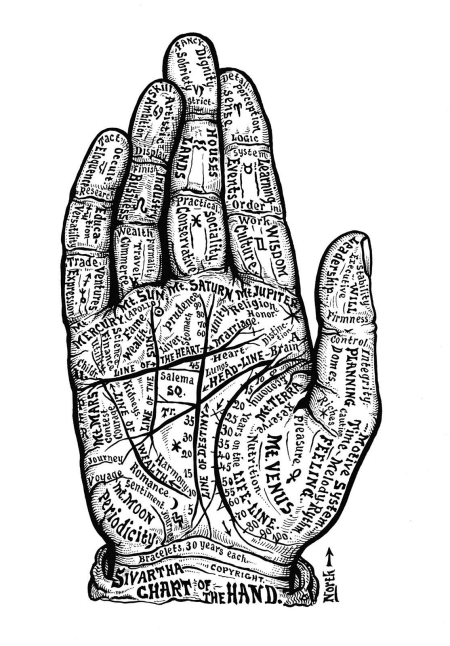
\includegraphics[scale=.5]{Tattoo}
  \end{center}


\myhighlight{Compass (Limb)}{sorcerer-tattoo-compass}

Always points towards true north.  

\myhighlight{Quill and Scroll (Back)}{sorcerer-tattoo-quill-scroll}

The quill can be removed as the Dagger, above - and given to someone else.  Anything that the other person writes with the quill will appear on the scroll tattooed on your Flesh ... painfully.  The writing disappears in Minutes.

\myhighlight{Eye (Palm)}{sorcerer-tattoo-eye}

The tattooed can see through the eye as if it were one of their normal eyes

\myhighlight{Rope (Neck, Arms, Legs, Torso}{sorcerer-tattoo-rope}

As Dagger above, 25m of rope. Needs to be completely rewound around the person to return to being a tattoo.


\myhighlight{Mermaid (chest or neck)}{sorcerer-tattoo-mermaid}

The Philosopher inscribes this tattoo on you and a \mylink{Wizard Sigil}{research-sigil-wizard} on a different object (usually a ship in a bottle or a scrimshawed whale bone).  You do not need to breathe to stay alive - you draw breath instead from the area immediately around the object.  This means that if the object is immersed in water, or sealed in an airtight container, you will suffocate.

\mysubsection{Sigils}{research-inscription-sigils}

Sigils are runes etched into surfaces.  Sigils glow slightly and exude arcane mystery, and are really obvious to everyone Nearby - but what the rune does can only be interpreted with a successful Skill:Lore check.  The creation of a new Sigil causes any previous Sigils of the same type created by the Philosopher to vanish.

A Sigil you encounter may be lifeless.  Sigils remain even after their magic is exhausted; only the sorcerer who created the Sigil can erase it from existence by placing a finger on it and reading its name aloud (note: the finger does not need to be attached to the hand, and the finger doesn't have to have flesh on it).  The sorcerer who etched the Sigil knows its "true name", otherwise you can figure it out with a successful Skill:Lore roll (if you fail your roll, you can try again next Session).

Unless otherwise specified, a Sigil can only be placed on something that is generally immobile and not alive - a door, a wall, the floor, a statue, etc.  Philosophers are immune to their own Sigil's effects where appropriate. 

\newpage 

\large{\mybold{Iron Sigils}}\normalsize

\example{
   1 Research \& 100\FE
}


\myanchor{\mybold{Chaining Sigil}}{research-sigil-chaining}  

A Chaining Sigil can be scribed and "married" to another Sigil.  The Chaining Sigil must be created at the same time as its partner Sigil.  If a Chaining Sigil is erased by the person who inscribed it, the Sigil it is partnered with will immediately manifest. The Sigil is permanent until erased.

\myanchor{\mybold{Talking Sigil}}{research-sigil-talking} 

When anyone comes Close to an object with a Talking Sigil on it, it will yell out a number of words at ear-splitting volume.  It will repeat these words a number of times, depending on the Research spent.  The Sigil is permanent until erased.

Each additional word/time you want the Talking Sigil to speak, you must spend an additional +1 Research/+100\FE.


\myanchor{\mybold{Warding Sigil}}{research-sigil-warding}

This glyph can only be placed on something that is closed : a book, a lock, a chest but not a sword in a scabbard or someone's mouth (Arbiter's discretion).  If the warded item is opened, the Sigil immediately becomes lifeless.

When anyone comes Close to an item with a Warding Sigil on it, they must Save or move somewhere Nearby, back the way they came.  The Sigil is permanent until erased.

For each 1 Research/100\FE you spend past the initial cost, the Warding Sigil effects a -1 modifier on the Save.


\myanchor{\mybold{Wizard Sigil}}{research-sigil-wizard}

The most basic Sigil, necessary to prepare a weapon, object, or person as a receptacle for magic.  The Sigil is permanent until erased.


\large{\mybold{Silver Sigils}}\normalsize


\example{
   3 Research \& 300\AG
}


\myanchor{\mybold{Cursing Sigil}}{research-sigil-cursing}

This Sigil can only be created with the help of a Mystic, who must use Cunning to create the \mylink{Malison}{occultism-malison} that resides in the Sigil.  When anyone comes Close to an object with the Sigil on it, they must Save vs. Hexes or fall victim to the curse. If there is more than 1 target, they should hold a Luck contest.  The Sigil becomes lifeless after it delivers its curse.

For each 1 Research/100\AG you spend past the initial cost, the Cursing Sigil affects a -1 modifier on the Save.


\myanchor{\mybold{Elemental Sigil}}{research-sigil-elemental}

When anyone comes Close to an object with an Elemental Sigil on it, they are dealt 4 elemental damage.  The inscriber chooses the elemental type (lightning, fire, etc).  Save for half damage.  The Sigil becomes lifeless after it delivers its damage.

For each 1 Research/100\AG you spend past the initial cost, the Elemental Sigil deals +4 damage


\myanchor{\mybold{ Petrifying Sigil}}{research-sigil-petrifying}

When anyone comes Close to a Petrifying Sigil, they must Save or become Paralyzed.  The duration of the paralysis lasts until the Sigil is erased. You age while you are paralyzed.

\myanchor{\mybold{Portal Sigil}}{research-sigil-portal}

These must be placed on doors, gates, or entrances.  A Portal Sigil is placed on the threshold or top of one doorway and a Wizard Sigil is placed on another; the two doors are connected as if they are the same door.  Someone stepping through the Portal Sigil side will exit through the \mylink{Wizard Sigil}{research-sigil-wizard} side (but not vice-versa).  The Sigil is permanent, but erasing either Sigil closes the doorway and makes the Portal Sigil lifeless (if the Wizard Sigil is erased).

\large{\mybold{Gold Sigils}}\normalsize


\example{
   5 Research \& 500\AU
}



\myanchor{\mybold{ Erasing Sigil }}{research-sigil-erasing}

When anyone comes Close to an Erasing Sigil, they must Save or suffer one of the effects below (roll a d6 for each person affected):

\mynumlist {
  \item Erases the spells etched in a sorcerer's mind
  \item Erases everything in a person's backpack
  \item Erases a person's armor and weapons (magic items get an additional Save)
  \item Erases all coins a person is carrying
  \item Erases a person's Grit, bringing it to zero
  \item Erases a person's Flesh and they are Dying
}

For each 1 Research/100\AU you spend past the initial cost, the Erasing Sigil affects a -4 modifier on the Save.  The Sigil is permanent until erased. 


\myanchor{\mybold{Remembrance Sigil}}{research-sigil-remembrance}

This Sigil can only be created with the help of a Spriggan, who will place one of the \mylink{Obliterated}{forgotten-obliterated} inside of the Sigil.  The maximum \HD of the creature starts at 2; for each 1 Research/100\AU you spend past the initial cost, this maximum is increased by +1.

Anyone other than the Sorcerer or Spriggan who comes Close to the Remembrance Sigil will cause the Obliterated to come forth - very pissed off - and immediately attack.  It will continue attacking as long as anyone is within Combat range (Close, Nearby, Far-Away, or Distant) - but it won't pursue anyone.  The Obliterated will return to its Sigil if there is no one to fight (this heals all damage and removes all negative effects).  If the Obliterated is slain, the Sigil will become lifeless.

\cbreak


\myanchor{\mybold{Revisitation Sigil}}{research-sigil-revisitation}

The Revisitation Sigil is scribed as normal (usually on a floor in the sorcerer's laboratory) and a \mylink{Chaining Sigil}{research-sigil-chaining} is placed on another portable item.  When the Chaining Sigil is erased, the Sorcerer is transported to the location of the Revisitation Sigil.  

For each 1 Research/100\AU you spend past the initial cost, you can bring 1 other Ally with you.  The Revisitation Sigil is permanent until erased, and can be bound to a new Chaining Sigil when its original partner is erased.


\newpage
